% !TEX root = tesis.tex

% arara: lualatex: { draft: yes }
% arara: biber if changed (toFile('refs.bib'))
% arara: --> || found ('log', 'Please \\(re\\)run Biber')
% arara: makeindex: { files: [ ejemplo.idx, names.idx ] }
% arara: --> if changed ('idx') || missing ('ind')
% arara: lualatex until !found('log', '\\(?(R|r)e\\)?run (to get|LaTeX)')
% arara: --> { synctex: on }

\documentclass{tesisFC}

%PAQUETES
%para los ejemplos
\usepackage{lipsum}%texto de demostración
\usepackage{xcolor}
\usepackage{tikz}
\usepackage{pgfplots}
\usepackage[autostyle]{csquotes}%recomendado para usar junto con biblatex
\usepackage[backend=biber,defernumbers,style=alphabetic,giveninits=true]{biblatex}%debe estar después del paquete de idiomas


%este no es recomendado sólo se carga para un ejemplo que muestra porqué
\ifpdftex
\usepackage[all,cmtip]{xy}
\fi

%este es recomendado, pero debe ser el último en casi todos los casos
\usepackage[colorlinks]{hyperref}
%para quitar el color de los links sustituir colorlinks por hidelinks


%BIBLIOGRAFÍA
\addbibresource{refs.bib}


%ÍNDICES Y GLOSARIOS
\makeindex
\makeindex[names]
%\makeglossary[acro]
%\makeglossary[simb]


%FLOTANTES
%subfloats en ambiente figura
\newsubfloat{figure}
%un nuevo flotante para diagramas
\newcommand{\diagramname}{Diagrama}
\newcommand{\listdiagramname}{Índice de Diagramas}
\newlistof{listofdiagrams}{dgm}{\listdiagramname}
\newfloat{diagram}{dgm}{\diagramname}
\newlistentry{diagram}{dgm}{0}
\newsubfloat{diagram}


%NUEVOS OPERADORES Y DELIMITADORES
\DeclareMathOperator{\id}{Idem}
\DeclarePairedDelimiter{\abs}{\lvert}{\rvert}
\providecommand\given{}%por si no está definido
\newcommand\SetSymbol[1][]{%
  \nonscript\:#1\vert%
  \allowbreak%
  \nonscript\:
  \mathopen{}}
\DeclarePairedDelimiterX\Set[1]\{\}{%
  \renewcommand\given{\SetSymbol[\delimsize]}#1}

%NUEVO ESTILO PARA ''TEOREMAS''
%estilo y "teoremas" adicionales
\newtheoremstyle{axioma}% nombre del estilo
{3pt}% espacio arriba
{3pt}% espacio abajo
{\itshape}% fuente del cuerpo
{0pt}% sangrado
{\bfseries}% fuente del nombre del teorema
{\newline}% puntuación después del nombre
{.5em}% espacio después del nombre
{\thmname{#1}\thmnote{ #3}}%

\theoremstyle{axioma}
\newtheorem{axioma}{Axioma}


%LIBRERIAS Y CONFIGURACIÓN DE TIKZ Y PGF
\usetikzlibrary{cd,calc,shadings,decorations.fractals,lindenmayersystems,math,datavisualization,datavisualization.formats.functions}
\pgfplotsset{width=6cm,compat=1.17}


%AMBIENTES (con luaLaTeX)
\ifluatex%
\setmathfont{GFS Neohellenic Math}[version=sansmath]
\setsansfont{GFS Neohellenic}
\setmathfont{XITS Math}[range=scr]
\newcounter{sans}
\newenvironment{sans}[1][]% environment name
{% begin code
  \par\vspace{\baselineskip}\sffamily\mathversion{sansmath}\noindent
  \refstepcounter{sans}%
  \textbf{Este texto está en sans \thesans\ #1}\ignorespaces%
}%
{% end code
  \par\vspace{\baselineskip}%
  \noindent\ignorespacesafterend%
}
\fi

%Información para la portada
\title{Título del trabajo}
\author{Nombre del alumno}
\date{2021}
\facultad{Ciencias}
\grado{Grado a obtener}
\tipo{tesis}
\tutor{Grado y nombre}
\logouni{unam}
\logofac{fc}


\begin{document}

\frontmatter%
\portadatesis%

%CONTENIDOS
\tableofcontents*
\clearpage
\listoffigures%
\clearpage
\listofdiagrams%


\mainmatter%
% !TEX root = tesis.tex

\chapter{Un poco de memoir}


\section{Lo básico}
La clase \texttt{tesisFC} tiene como base a \textit{memoir}. La motivación es poder configurar de manera fácil los ascpectos del documento sin tener que usar paquetería adicional. Así, cuando el usuario cargue un paquete es poco probable que cause alguna incompatibilidad.¡

\textit{Memoir} es una clase configurable, es decir, no hace falta cargar paquetes adicionales para hacer un diseño completo de cómo se verá nuestro
documento. Además puede servir tanto para \textit{book} como para \textit{article} la opción por defecto es una salida estilo \textit{book}, para cambiar al diseño estilo \textit{article} basta poner la opción \texttt{article} como opción a la clase. A diferencia de las clases
estándar donde hacer un cambio de \textit{book} a \textit{article} seguramente causará problemas (por ejemplo \verb|\chapter{...}| no está
definido en article), en \textit{memoir} no existe ese problema. Otra ventaja inmediata es que el ambiente \texttt{abstract} estará definido para \textit{book}.

La tabla de contenidos esta formada por el comando
\verb|\tableofcontents*|. Esta versión con estrella es única de memoir y su
utilidad es que no aparezca una entrada para la tabla de contenidos en la
tabla de contenidos.

Otra ventaja de \textit{memoir} es que no hace falta redefinir
\verb|\cleardoublepage| para que las páginas pares ``vacías'' antes de un
nuevo capítulo estén en blanco. La clase ya lo hace por defecto. Además, la
clase tiene las opciones \texttt{openright} para que los capítulos empiecen
en las paginas impares, \texttt{openleft} para que empiecen en las pares y
\texttt{openany} para que empiecen en la siguiente página sin importar su
paridad.

Memoir tiene predefinidos muchos estilos de capítulo, em este documento se está usando \texttt{madsen}. Memoir tiene
definidos muchos más estilos de salida por defecto, estos pueden verse en
\url{http://www.ebookation.com/wp-content/uploads/2010/03/memoirchapstyles.pdf}

Modifique el tamaño y la posición de la caja de texto para obtener una linea de texto suficientemente grande como evitar tantos cortes de palabra, pero no ta grande como para que sea difícil pasar de una lína a otra.

Si notan como está formado un libro, el bloque de texto no está centrado
en la página. Comúnmente el margen de la espina (donde se juntan las
páginas de un libro) es la mitad que el margen de la orilla (el opuesto a
la espina). Lo mismo sucede con los margenes superior e inferior, donde el
superior es más chico que el inferior. Tomamos en cuenta estos detalles en
la formación de este documento.

También cambié cabeceras y pies, esta vez fue mínimo pero aún así es
suficiente para ver cómo cambiar cabeceras y pies (ver archivo \texttt{.cls}).

Menciono de nuevo que \textit{memoir} es una clase configurable y tiene de
manera nativa capacidades mayores o iguales a
las de los siguientes paquetes
\begin{center}
  \autocols{c}{6}{l}{abstract, appendix, booktabs, ccaption, chngcntr, chngpage, enumerate, epigraph, framed, ifmtarg, index, makeidx, moreverb, needspace, newfile, nextpage, parskip, patchcmd, setspace, shortvrb, showidx, titleref, titling, tocbibind, tocloft, verbatim, verse}
\end{center}
También tiene las capacidades, aunque con comandos diferentes, de los siguientes paquetes
\begin{center}
  crop, fancyhdr, geometry, sidecap, subfigure, titlesec
\end{center}
Por último, la clase carga los siguientes paquetes
\begin{center}
  array, dcolumn, delarray, etex, iftex, tabularx, textcase (con la opción \texttt{overload})
\end{center}
Así que no hace falta cargar ninguno de estos, de esta manera es más fácil
tener compatibilidad de paquetes.

\textit{Memoir} puede crear índices de manera relativamente sencilla, en este ejemplo
haremos uno de términos o alfabético y uno de nombres. Para esto se escribió
en el preámbulo
\begin{flushleft}
  \verb|\makeindex|\\
  \verb|\makeindex[names]|
\end{flushleft}
luego una entrada en el índice de términos se crea con el comando
\verb|\index{término}| término\index{término}. Este índice puede crear
subtérminos de la siguiente manera subtérmino\index{término!subtérmino} y
uno más subsubtérmino\index{término!subtérmino!subsubtérmino} (ver código
fuente).

Ahora una entrada para el índice de nombres
Grothendieck\index[names]{Grothendieck}. Nota que en este índice se
específico que pertenece al índice de nombres con el parámetro opcional
\texttt{[names]}.

Al final del archivo principal se puede ver cómo se imprimieron.


\section{Un poco más}
Primero veamos cómo hacer subfiguras con memoir, es decir, sin usar el paquete
\texttt{subfigure} o \texttt{subcaption}. Primero necesitamos escribir
\begin{flushleft}
  \verb|\newsubfloat{figure}|
\end{flushleft}
en el preámbulo. Este comando activará todo lo necesario para hacer
subfiguras, por ejemplo en la figura~\ref{fig:vect} hay
una forma de hacerlas usando el comando \verb|\subcaption{...}| para poner
los subtítulos correspondientes. También es posible hacer como en el
siguiente ejemplo
\begin{figure}
  \centering
  \subbottom[Primera]{%
    \includegraphics[width=0.3\linewidth]{example-image-a}}
  \subbottom[Segunda]{%
    \includegraphics[width=0.3\linewidth]{example-image-b}}
  \subbottom[Tercera]{%
    \includegraphics[width=0.3\linewidth]{example-image-c}}
  \caption{Muchas figuras}
\end{figure}
Nota que no hay archivos aparte para las figuras que usamos. Estas ya están
instaladas con nuestra distribución y podemos usarlas como lo hicimos.
Además como su nombre lo indica, un \textit{float} está flotando en la
página y \LaTeX{} decidirá cual es el mejor lugar para ponerlo. Otro ejemplo
de flotante es una tabla. Las opciones para la ubicación de flotantes son
las siguientes.
\begin{description}
  \item [h] trata de poner el flotante donde fue creado.
  \item [t] lo pone en la parte superior de la página.
  \item [b] lo pone en la parte inferior de la página.
  \item [p] lo pone en una página especial para flotantes.
  \item [h!] se esfuerza más en poner el flotante donde fue creado.
\end{description}
La sintaxis para especificar la posición es \verb|\begin{figure}[...]|.

También es posible crear nuevo flotantes, nosotros hemos hecho un flotante
para diagramas en el preámbulo. Así podemos poner diagramas en una versión
similar a la de figura.
\begin{diagram}
\centering
\begin{tikzpicture}[commutative diagrams/every diagram]
  \node (P0) at (90:2.3cm) {\(X\otimes (Y\otimes (Z\otimes T))\)};
  \node (P1) at (90+72:2cm) {\(X\otimes ((Y\otimes Z)\otimes T))\)} ;
  \node (P2) at (90+2*72:2cm) {\makebox[5ex][r]{\((X\otimes (Y\otimes Z))\otimes T\)}};
  \node (P3) at (90+3*72:2cm) {\makebox[5ex][l]{\(((X\otimes Y)\otimes Z)\otimes T\)}};
  \node (P4) at (90+4*72:2cm) {\((X\otimes Y)\otimes (Z\otimes T)\)};
  \path[commutative diagrams/.cd, every arrow, every label]
    (P0) edge node[swap] {\(1\otimes\alpha\)} (P1)
    (P1) edge node[swap] {\(\alpha\)} (P2)
    (P2) edge node[swap] {\(\alpha\otimes 1\)} (P3)
    (P4) edge node {\(\alpha\)} (P3)
    (P0) edge node {\(\alpha\)} (P4);
\end{tikzpicture}
\caption{¡Pentagonator!}
\end{diagram}
También es posible aprovechar el espacio del margen como apoyo para las figuras.
\begin{marginfigure}
\centering
  \begin{tikzpicture}
    \draw (0,0) circle (5mm);
  \end{tikzpicture}
  \caption{Un circulo en el margen}
\end{marginfigure}

Por último en el código de este documento se puede ver que todas las
figuras tienen inmediatamente después del inicio del ambiente el comando
\verb|\centering|, debe ser este y no usar el ambiente \texttt{center}
para evitar espacios verticales no deseados. Además, como esto se hizo en
cada figura pudo haberse configurado en el preámbulo con el siguiente
comando
\begin{flushleft}
  \verb|\setfloatadjustment{figure}{\centering}|
\end{flushleft}
que también se puede usar en tablas, figuras al margen y los flotantes que
se hayan creado.


\section{Falta desarrollar mejor}
Memoir puede crear glosarios de una forma muy similar a los índices. En este
documento se crearon una lista de acrónimos y una de símbolos para
ejemplificar cómo se hacen. En el preámbulo se escribió
\begin{flushleft}
  \verb|\makeglossary[acro]|\\
  \verb|\makeglossary[simb]|
\end{flushleft}
Luego un acrónimo HTML\glossary[acro]{HTML}{⟨HyperText Markup Language} y un
símbolo \(c\)\glossary[simb]{\(c\)}{Una constante importante}. Por último,
al finas del documento principal verás como se imprimió cada uno.

La dificultad que encuentro en la creación de glosarios es la compilación.
Para esto también se usará \textit{makeindex}, pero si se intenta correr
este programa en alguno de los archivos para crear glosarios, por ejemplo
\begin{flushleft}
  \verb|makeindex acro.glo|
\end{flushleft}
se generaran muchos errores. Entonces, para lograr hacer estos glosarios se
necesita un archivo de configuración \texttt{basic.gst} que encontrarás en
los archivos de este proyecto y con esto la cadena de compilación que se uso para los glosarios de este documento es
\begin{flushleft}
  \verb|...|\\
  \verb|makeindex -s basic.gst -o acro.gls acro.glo|\\
  \verb|makeindex -s basic.gst -o simb.gls simb.glo|\\
  \verb|lualatex MiDocumento.tex|
\end{flushleft}
como no estoy seguro como llamar un archivo de configuración externo en
\texttt{arara} tuve que correr los dos \texttt{makeindex} en la terminal.

Acabo de hacer una prueba en overleaf y tristemente no soporta esta
construcción  de glosarios. Por lo tanto sugeriré el paquete
\texttt{glossaries} o su versión extendida \texttt{glossaries-extra}. La
versión extendida tiene muchas capacidades con el método \texttt{bib2gls} pero
tampoco es soportado por overleaf. Por lo que para hacer glosarios en overleaf
hay que usar la versión simple de \texttt{glossaries} que debería ser
suficiente para una tesis.

% !TEX root = ejemplo.tex

\chapter{Fuentes}
Para las fuentes del documento he escogido los paquetes \texttt{fontspec} y
\texttt{unicode-math} en el caso de compilar con Lua\LaTeX. Si la
compilación es con pdf\LaTeX{} se usarán los paquetes \texttt{inputenc} y
\texttt{fontenc}.

La ventaja de \texttt{fontspec} y \texttt{unicode-math} es que posible
cambiar fuentes de manera fácil en partes del documento, pero deberá ser
compilado con Xe\LaTeX{} o con Lua\LaTeX, el último siendo el método
recomendado. Con esto se podrán usar caracteres unicode en cualquier parte
de texto, por ejemplo en una ecuación centrada (para que aparezcan las
ecuaciones compila con Lua\LaTeX.)
\ifluatex%
\[
  ∀ε>0∃δ>0(|x-y|<δ ⇒ |f(x)-f(y)|<ε)
\]
\else
\ifpdftex%
\begin{center}
\textcolor{red}{La compilación con pdf\LaTeX{} no permite mostrar este
ejemplo.}
\end{center}
\fi
\fi
o en una línea de texto%
\ifluatex%
\(∀ε>0∃δ>0(|x-y|<δ ⇒ |f(x)-f(y)|<ε)\).
\else
\ifpdftex%
\textcolor{red}{La compilación con pdf\LaTeX{} no permite mostrar este
ejemplo.}
\fi
\fi
Las letras griegas, por ejemplo, no necesitan estar en modo matemático para
funcionar
\ifluatex%
αβγδφψ
\else
\ifpdftex%
\textcolor{red}{La compilación con pdf\LaTeX{} no permite mostrar este
ejemplo.}
\fi
\fi
(ver código fuente ignorando los condicionales para cada tipo de
compilación).

La fuente que fue escogida para este texto es \textit{Stix Two}. Esta fuente
tiene como objetivo servir como un estándar para la preparación, publicación
e impresión de textos científicos. Es impulsada y usada por la \textit{AMS}
(matemáticas), \textit{ACS} (química), \textit{AIP} y \textit{APS} (física),
\textit{IEEE} (ingeniería) y Elsevier. Por lo tanto, tiene un conjunto de
símbolos sumamente extenso.

Para nuestros ejemplos, con Lua\LaTeX, se cambiara el tipo de fuente sans
por GFS Neohellenic. No es recomendable usar muchos tipos de fuente en un
documento, pero como esto es un ejemplo haremos dicho cambio. Como distintas
fuentes tienen distintos tamaños, al combinar dos de ellas es muy posible
crear una inconsistencia en los tamaños. Para evitar esto use la opción de
\texttt{fontspec} (ver preámbulo) \texttt{Scale=MatchUppercase}. Este
paquete puede hacer muchas modificaciones a los atributos de una fuente y no
veremos más de esos atributos. En el preámbulo está la definición de un
ambiente donde la fuente se cambia:
\ifluatex%
\begin{sans}%
\label{textosans}
  \lipsum[1][1-3]
  \[
    \prod_{i\in I}A_i\ne\emptyset
  \]
\end{sans}
Como el objetivo fue cambiar la fuente sans el cambio también se hará al usar
\verb|\textsf{...}| y \verb|{\sffamily ...}| como podemos ver a continuación
\textsf{cambio de fuente
\mathversion{sansmath}\(\forall\varepsilon>0\exists\delta>0(\ldots)\)}. Como
puede verse en el ejemplo lo que hace cambiar la fuente matemática es el
comando \verb|\mathversion{sansmath}| de \texttt{unicode-math}.
\else
\ifpdftex%
\begin{center}
\textcolor{red}{La compilación con pdf\LaTeX{} no permite mostrar este
ejemplo.}
\end{center}
\fi
\fi

Un ejemplo de dónde se hizo este tipo de cambios es en las Lecturas de Física
de Feynman. En este texto las figuras llevan un tipo de fuente diferente a la
del cuerpo.
\ifluatex%
\begin{figure}[h]
\mathversion{sansmath}
\centering
\begin{minipage}{0.4\linewidth}
\centering
\begin{tikzpicture}
  \draw[gray!70,->] (0,0) -- (3,0);
  \draw[gray!70,->] (0,0) -- (0,3);
  \draw[->] (0,0) -- (1,1.5) node[above] {\(x\)};
  \draw[->] (0,0) -- (2,0.5) node[right] {\(y\)};
  \draw[->] (0,0) -- (3,2) node[above] {\(x+y\)};
  \draw[dotted] (1,1.5) -- (3,2) -- (2,0.5);
\end{tikzpicture}

  \captionnamefont{\sffamily}
  \subcaption{\sffamily Suma de vectores}
  \label{fig:vect1}
\end{minipage}
\hfill
\begin{minipage}{0.4\linewidth}
\centering
\begin{tikzpicture}
  \draw[gray!70,->] (0,0) -- (3,0);
  \draw[gray!70,->] (0,0) -- (0,3);
  \draw[->] (0,0) -- (1,1.5) node[above] {\(x\)};
  \draw[->] (0,0) -- (2,0.5) node[right] {\(y\)};
  \draw[->] (1,1.5) -- node[right] {\(y-x\)} (2,0.5);
\end{tikzpicture}

  \captionnamefont{\sffamily}
  \subcaption{\sffamily Resta de vectores}
  \label{fig:vect2}
\end{minipage}
  \captionnamefont{\sffamily}
  \caption{\sffamily Operaciones con vectores}
  \label{fig:vect}
\end{figure}
\else
\ifpdftex%
\begin{center}
\textcolor{red}{La compilación con pdf\LaTeX{} no permite mostrar este
ejemplo.}
\end{center}
\fi
\fi

Como no está pensado para que así sea la salida de todas las figuras no se
hizo la definición en el preámbulo. Para dicho cambio se debe escribir
\verb|\captionnamefont{\sffamily}| para cambiar el tipo de fuente de la
palabra ``Figura'' y su número. Para cambiar el delimitador, que en este caso
son dos puntos se usa \verb|\captiondelim{: }|. Para cambiar el tipo de
fuente del título de las figuras se usa \verb|\captiontitlefont{\sffamily}|.
Con esto es fácil hacer una configuración de la salida de los títulos de
figuras y tablas, también se podría cambiar el tamaño de la fuente o poner
alguna palabra en específico.

Otra ventaja del manejo de fuentes de Xe\LaTeX{} y Lua\LaTeX{} es que las
fuentes instaladas en nuestra sistema estarán disponibles para su uso en
documentos de \LaTeX{}. Por ejemplo si quisiéramos que nuestro documento
estuviera escrito en Arial simplemente hay que escribir
\begin{flushleft}
  \verb|\setmainfont{Arial}|
\end{flushleft}
contrario a la forma en la que hace pdf\LaTeX{} donde habría que usar el
código de la fuente y en muchos casos es difícil encontrar dicho código.
Además que las fuentes disponibles de esa forma son relativamente pocas.
Para dar una idea de la disponibilidad de fuentes con Xe\LaTeX{} y
Lua\LaTeX{} basta ver las fuentes disponibles en overleaf \url{https://www.overleaf.com/latex/examples/fontspec-all-the-fonts/hjrpnxhrrtxc}.
Seguramente en tu sistema habrá un conjunto de fuentes disponibles grande.

\ifluatex%
Un comentario acerca de \texttt{unicode-math} es que permite usar una
fuente específica para cada alfabeto. El ejemplo en este texto es cambiar la
fuente script, que tanto en \textit{Stix two} como muchas otra fuentes es
igual a la caligráfica. Con \texttt{unicode-math} es suficiente cargar una
fuente con el alfabeto que nos guste, sólo para el rango que la queremos.
Aún cuando en un principio no es necesario tener tantos alfabetos matemáticos
diferentes, en teoría de categorías he visto una notación que aunque no es
estándar (creo que aún no hay ningún estándar) parece dar coherencia. Las
categorías pequeñas y localmente pequeñas se denotan con letras en negritas
\(\mbfA \), \(\symbf{Con}\),\ldots categorías más grandes se denotan con
letras caligráficas \(\mathcal{X}\), \(\symcal{Y}\), etc. y categorías
especiales como topos se denotan con letras script como \(\symscr{E}\).

En el código se puede notar que se han usado diferentes sintaxis para los
alfabetos, que \texttt{unicode-math} se encargará de mapear al símbolo
correcto. Por ejemplo, las formas de obtener la letra ``A'' en negritas es
como símbolo definido por un alfabeto \verb|\mbfA|, como comando de
\texttt{unicode-math} (es la forma recomendada) \verb|\symbf{A}| o como en
la forma ``tradicional'' \verb|\mathbf{A}|.
\ifpdftex%
\begin{center}
  \textcolor{red}{Este párrafo usa comandos específicos de \texttt{unicode-math} y mandará erroes si se compila con pdf\LaTeX.}
\end{center}
\fi
\fi

Algo que hay que notar es que el soporte de rango y versiones en
\texttt{unicode-math} es aún experimental, por lo que para que funcione como
en este ejemplo se debe escribir primero la versión
\verb|\setmathfont{GFS Neohellenic Math}[version=sansmath]|
y luego el rango \verb|\setmathfont{XITS Math}[range=scr]|. De lo contrario
GFS Neohellenic reescribiría el rango y no lograríamos lo que se quería
mostrar.

% !TEX root = ejemplo.tex

\chapter{Paquetes en la clase}

\section{amsmath y mathtools}
Aunque en el título de la sección se menciona \texttt{amsmath} en la clase
sólo se carga el paquete \texttt{mathtools}. Esto se debe a que
\texttt{mathtools} carga al paquete \texttt{amsmath}, así lo podemos pensar
como una extensión. De manera más precisa \texttt{mathtools} es resultado de
corregir algunos ``bugs'' de \texttt{amsmath} y añadir algunas otras funciones.

Un ejemplo específico de estos paquetes es la creación de operadores. Por
ejemplo, para escribir el supremo del conjunto \(A\) se debe escribir
\verb|\sup A| y su resultado es \(\sup A\), de donde es claro que los
operadores están en letras \textit{upright}. Ya están definidos los
operadores más comunes, pero si se quisiera definir uno nuevo se escribe en
el preámbulo \verb|\DeclareMathOperator{\id}{Idem}| para definir los
idempotentes de un anillo, por ejemplo \verb|\id(R)| genera \(\id(R)\).
Además de esto están los ambientes matemáticos como \texttt{align},
\texttt{gather}, \texttt{cases}, etc.

Una función de \texttt{mathtools} que no tiene \texttt{amsmath} es la creación
de delimitadores que se pueden ajustar al tamaño del contenido, por ejemplo
para hacer un delimitador para el valor absoluto se escribe
\verb|\DeclarePairedDelimiter\abs{\lvert}{\rvert}| este
tiene un argumento más que el operador ya que hay que decir qué símbolo
``abre'' y que símbolo ``cierra''. La deferencia de este comando se puede
apreciar con el código \verb!|\sum_{i=1}^{n}a_1|!,
\verb|\lvert\sum_{i=1}^{n}a_1\rvert|, \verb|\abs{\sum_{i=1}^{n}a_1}| y
\verb|\abs*{\sum_{i=1}^{n}a_1}|, que su salida es, respectivamente,
\[
  |\sum_{i=1}^{n}a_1| \quad \lvert\sum_{i=1}^{n}a_1\rvert \quad
  \abs{\sum_{i=1}^{n}a_1} \quad \abs*{\sum_{i=1}^{n}a_1}
\]

También podemos hacer conjuntos con delimitadores y la línea de ``tal que''
que crezcan correctamente (ver su definición en \texttt{ejemplo.tex})
\[
  \Set*{ x \in X \given \frac{\sqrt{x}}{x^2+1} > 1 }
\]


\section{amsthm}
Este paquete provee mejoras útiles para las definiciones de teoremas
(\LaTeX{} puede crea teoremas sin necesidad de paquetes) y
define un ambiente de demostración (esto no lo hace \LaTeX{}). Con este
paquete se pueden usar y definir estilos de teoremas de forma fácil. En la calse se definieron los siguinetes ambientes:
\begin{center}
  \autocols{c}{3}{l}{\texttt{definicion}, \texttt{lema}, \texttt{teorema}, \texttt{proposicion}, \texttt{corolario}, \texttt{observacion}}
\end{center}
Con la salida esperada del nombre del ambiente.

\begin{definicion}
  Una función \(f\colon X\to Y\) es continua si para cualquier abierto
  \(V\subseteq Y\) se tiene que \(f^{-1}(V)\subseteq X\) es abierto.
\end{definicion}

\begin{teorema}[Fermat]%
\label{teo:fermat}
  La ecuación \(x^n + y^n = z^n\) con \(n\geq 3\) no tiene soluciones no triviales en \(\mathbb{Z}\).
\end{teorema}
\begin{proof}
  He descubierto una demostración maravillosa de esto, que este margen es
  demasiado estrecho para contener.
\end{proof}

Se modificó el estilo del ambiente demostración para que su salida sea similara a la de los resultados —Una demostración es tan importante como el
enunciado—. Nuestra redefinición del ambiente de demostración tiene lo necesario para comportarse bien con el símbolo\(\qed \). Es decir, cuando se termina una demostración con una ecuación u otro tipo de ambiente habrá
un espacio vertical indeseado entre el final del texto y el símbolo de fin de la demostración. Este espacio se evita con el comando \verb|\qedhere|, pero si el ambiente no cuenta con la definición correcta seguirá
apareciendo este espacio vertical. Un ejemplo de cómo funciona \verb|\qedhere|, para mostrar la diferencia se han hecho dos demostraciones iguales

\begin{teorema}
  Un resultado importante.
\end{teorema}
\begin{proof}
  Se sigue de la siguiente ecuación (sin usar \verb|\qedhere|)
  \[
    \sum_{n\geq 1}\frac{1}{n}=-\frac{1}{12}.
  \]
\end{proof}
\begin{proof}[¿Es otra demostración?]
  Se sigue de la siguiente ecuación (usando \verb|\qedhere|)
  \[
    \sum_{n\geq 1}\frac{1}{n}=-\frac{1}{12}. \qedhere
  \]
\end{proof}

Cada ``teorema'' nuevo crea un contador. En este ejemplo la cuenta de
teoremas se reiniciará al iniciar un nuevo capítulo, este es el efecto del
comando opcional \texttt{[chapter]} en la definición de \texttt{teorema}.
Además, el contador de las definiciones será el mismo que el de los teoremas
(notar que aparece definición 4.1, teorema 4.2), esto lo hace el parámetro
opcional \texttt{[teorema]} en la definición de \texttt{definicion}. Esta
cuenta de teoremas sirve para hacer referencia a resultados o definiciones
en el futuro. Al teorema le pusimos una etiqueta con el comando
\verb|\label{teo:fermat}| que luego se puede hacer referencia con
\verb|\ref{{teo:fermat}}|. Una buena práctica es separar la referencia de la
palabra anterior con un espacio irrompible \verb|~|, de esta forma cuando
escribimos ``por el teorema~\ref{teo:fermat}'' \LaTeX{} no podrá romper un
renglón dejando la palabra ``teorema'' en un renglón y el número ``4.2'' en
otro.

Nota que el estilo \texttt{plain} pone el cuerpo del teorema en itálicas
mientras que el estilo \texttt{definition} no, como puede verse en el
enunciado de la definición y de los teoremas.

En el preámbulo de \texttt{ejemplo.tex} está un ejemplo de cómo crear un
estilo nuevo de ``teorema''. En este se creó un ambiente para los axiomas
usando un estilo diferente que llevará una cuenta independiente de las
definiciones anteriores, pues no aparece la opción \texttt{[teorema]} en su
definición.

\begin{axioma}
  Para toda \(f\colon D\to R\) existe una y sólo una \(b\in R\) tal que para
  cualquier \(d\in D\)
  \[
    f(d)=f(0)+d\cdot b.
  \]
\end{axioma}

Adicionalmente, se podría hacer las definiciones de estos ambientes de
teorema y demostración como un nuevo ambiente. El ejemplo, compilando con
Lua\LaTeX, con tipo de letra sans en~\ref{textosans} tiene lo necesario para
crear un ambiente y contador con las características como las de los
ambientes de \texttt{amsthm}.

Finalmente, otro paquete común para el manejo de teoremas y demostraciones
es \texttt{ntheorem}. Cada uno tiene sus ventajas y desventajas y no es
fácil elegir uno sobre otro. En este documento se eligió \texttt{amsthm}
porque es (posiblemente) el más común.


\section{babel y polygossia}%
\label{sec:babel}
Para el soporte de idiomas elegimos \texttt{polygossia} en caso de compilar
con Lua\LaTeX{} y \texttt{babel} en caso de compilar con pdf\LaTeX.

En el caso de \texttt{babel} se carga con las opciones \texttt{spanish} y
\texttt{mexico}. La opción \texttt{mexico} hace una localización más similar
a la que se usa en México, como su nombre lo indica. Entre las cosas que
hace podemos mencionar que cambia el nombre ``cuadro'' por ``tabla'',
prioriza comillas y usa el punto decimal en lugar de la coma como puede
verse \(\pi=3.141592\ldots \)

Al usar el idioma español \texttt{babel} se encargará de traducir todo, por ejemplo la palabra ``capítulo'' o ``figura'' como se puede ver en el documento. También traduce y acentúa los operadores, por ejemplo \(\max A\) o \(\lim f\).%
\ifpdftex%
Pero en algunos casos se decidió crear un comando nuevo como en el caso del
seno:
\[
  \sin(\alpha)\ne\sen(\alpha)
\]
\fi

Otra opción para el manejo de idiomas en Xe\LaTeX{} o Lua\LaTeX{} es
\texttt{polyglossia}. Este paquete se creó cuando \texttt{babel} había
dejado de tener mantenimiento con el objetivo de simplificar su trabajo en
estos motores. Este paquete también tiene una variante \texttt{mexico},
además de que se puede elegir un poco más el comportamiento de los
operadores con las opciones:
\begin{description}
  \item[\texttt{accented}] para acentuar los operadores como \texttt{babel}.
  \item[\texttt{spaced}] para dar un espacio corto entre el operador y el objeto al que se le aplica, de nuevo, como \texttt{babel}.
  \item[\texttt{all}] para hacer las dos anteriores más la localización de \verb|\sin| \verb|\tan| \verb|\sinh| y \verb|\tanh|.
  \item[\texttt{none}] para no hacer ninguna localización.
\end{description}
De esta forma se cargó polyglossia \texttt{polyglossia} con la siguiente
configuración
\begin{flushleft}
  \verb|\usepackage{polyglossia}| \\
  \verb|\setdefaultlanguage[spanishoperators=all]{spanish}|
\end{flushleft}

Tanto \texttt{babel} como \texttt{polyglossia} son buenas opciones para el
manejo de idiomas y es difícil elegir uno sobre el otro. En el caso de
compilar con Lua\LaTeX{} se decidió usar \texttt{polygossia} ya que es fácil
ajustar el sangrado de los párrafos. Esto es, en español el primer párrafo
despues del título de un capítulo, sección, etc. no debería estar sangrado.
\LaTeX{} toma esto en cuenta, pero \texttt{babel} sobreescribe este
comportamiento y sangra este primer párrafo (compilar este documento con
pdf\LaTeX{} para ver la diferencia). Aunque \texttt{polygossia} hace lo
mismo es fácil evitar esto con el comando
\begin{flushleft}
  \verb|\PolyglossiaSetup{spanish}{indentfirst=false}|
\end{flushleft}
En \texttt{babel} usando español se supone que sí existe la posibilidad de
corregir esto (en otros idiomas no es posible), pero el manual no menciona
nada al respecto.


\section{microtype}
Este paquete habilita los aspectos micro-tipográficos del documento. Algunos
de ellos ya son hechos por \TeX{} como justificación y la separación
silábica (cortes de palabra). En general las opciones que se le pasaron a
este paquete sirven para calcular la expansión de letras, palabras y
permitir que algunos caracteres, como el guión de un corte de palabra,
salgan del margen. Algunas de estas mejoras se pueden hacer con
\texttt{fontspec}, por ejemplo poniendo la opción \texttt{LetterSpacing} al
cargar una fuente, pero hay que calcular las cosas manualmente. En cambio
\texttt{microtype} toma todas estas decisiones por nosotros y lo hace
de acuerdo al idioma que se la haya pasado a \texttt{babel}. El resultado es
un pdf que luce tipográficamente mejor.


\section{siunitx}
Este paquete tiene como objetivo implementar la escritura de cantidades
físicas de acuerdo con las reglas del sistema internacional de medidas\footnote{\url{https://www.bipm.org/en/measurement-units/}}. Aunque hay un desacuerdo con la forma de espaciar las cantidades y las unidades debido a la mala traducción del francés (idioma de la versión oficial del manual del sistema internacional de medidas) al inglés (idioma de donde se basaron para la creación del paquete). En el francés dice que deberían separase con un espacio y en el inglés dice que se separan con un \textit{thin space}. Así, el espaciado no es el correcto pero el error puede ser productivo ya que un menor espaciado crea una relación más estrecha entre cantidad y unidad. Algunos ejemplos de este paquete están en la siguiente tabla:
\begin{center}
  \begin{tabular}{lc}
    \toprule
    Comando & Resultado \\
    \midrule
    \verb|\ang{1;2;3}| & \ang{1;2;3}\\
    \verb|\si{\gram\per\cubic\centi\metre}| & \si{\gram\per\cubic\centi\metre}\\
    \verb|\si{kg.m/s^2}| & \si{kg.m/s^2}\\
    \verb|\SI{.23e7}{\candela}| & \SI{.23e7}{\candela} \\
    \verb|\SI[mode=text]{1.23}{J.mol^{-1}.K^{-1}}| & \SI[mode=text]{1.23}{J.mol^{-1}.K^{-1}} \\
    \verb|\SI[per-mode=symbol]{1.99}[\$]{\per\kilogram}| & \SI[per-mode=symbol]{1.99}[\$]{\per\kilogram} \\
    \verb|\SI[per-mode=fraction]{1,345}{\coulomb\per\mole}| & \SI[per-mode=fraction]{1,345}{\coulomb\per\mole}\\
    \bottomrule
  \end{tabular}
\end{center}


\section{biblatex}%
\label{sec:bib}
En principio no se eligió ningún paquete para crear la bibliografía del documento, pero el que nos parece recomendable es \texttt{biblatex}. Hay otros paquetes para formar la bibliografía de un texto, por ejemplo
\texttt{natbib} o \texttt{cite}.

Mientras que \texttt{natbib} y \texttt{cite} son muy parecidos, sólo cambian
algunas capacidades y \texttt{natbib} puede hacer técnicamente todo lo que
hace \texttt{cite} más algunas cuantas cosas; \texttt{biblatex} es muy
diferente a estos dos paquetes.

Como este es un texto ``local'' en el sentido que su código fuente no debe
cumplir los requerimientos de ningún \textit{journal} o editorial, entonces
es posible usar los paquetes que cada quien considere necesario. La
motivación principal para hacer este ejemplo con \texttt{biblatex} está
en el siguiente link \url{https://tex.stackexchange.com/a/25702/140456},
donde se explican las ventajas de biber sobre bibtex.

La construcción de la base de datos de referencias es básicamente la misma
para cualquier paquete de los anteriores. Hay herramientas gráficas útiles
para hacer esto como JabRef o Zotero.

El paquete \texttt{biblatex} puede manejar muchos tipos de entrada. En el
manual se describe el uso de los siguientes
\autocols{c}{5}{l}{%
  article, book, mvbook, inbook, bookinbook, suppbook, booklet, collection, mvcollection, incollection, suppcollection, dataset, manual, misc, online, patent, periodical, suppperiodical, proceedings, mvproceedings, inproceedings, reference, mvreference, inreference, report, set, software, thesis, unpublished, xdata, custom[a-f], conference, masterthesis, pdhthesis, techreport, www, artwork, audio, bibnote, commentary, image, jurisdiction, legislation, legal, letter, movie, music, performance, review, standard, video
  }
Son demasiados para dar una descripción breve, pero en el manual de
\texttt{biblatex} no sólo se describe para qué se usa cada una sino que
también algunos campos recomendados para algunas de ellas.

La lista de campos que se pueden usar en las entradas es demasiado larga para
escribirla aquí. De nuevo, en el manual se dan los campos disponibles junto
con una descripción breve.

También tiene una lista grade de formas de citación, las más comunes son
\verb|\cite{...}|, \verb|\parencite{...}|, \verb|\textcite{...}| y
\verb|\footcite{...}|. El estilo de las entradas bibliográficas y de la
citación se hacen mediante opciones del paquete. Como la lista de opciones
también es amplia haré referencia a la siguiente liga
\url{http://tug.ctan.org/info/biblatex-cheatsheet/biblatex-cheatsheet.pdf}
para tener una guía rápida de \texttt{biblatex}.

En este ejemplo hice un archivo \texttt{refs.bib} como base de datos de la
bibliografía. Para ``cargarlo'' hay que usar el comando
\verb|\addbibresource{refs.bib}|. Este comando sólo acepta un archivo, pero
se pueden cargar más escribiendo todo el comando con cada archivo
\texttt{.bib} que se quiera usar. Para imprimir la bibliografía se pone el
comando \verb|\printbibliography| donde se quiera tener la bibliografía. Por
ejemplo se puede imprimir una bibliografía por capitulo, por tipo
(artículo, libro, etc.), por alguna palabra clave, etc.

En principio sólo imprime las entradas que fueron citadas en el texto, si se
quiere imprimir una entrada que no fue citada se usa el comando
\verb|\nocite{label1,label2,...}| o si se quiere imprimir todas las entradas
del archivo \texttt{.bib} se usa \verb|\nocite{*}|.

Por último es recomendable usar el paquete \texttt{csquotes} junto con
\texttt{biblatex} para tener algunas facilidades en citas y ajustar las
comillas al idioma que se quiera. En este documento se uso junto con la
opción \texttt{autostyle} que carga el estilo de comillas del idioma que se
haya pasado a babel, es este caso español. Como puede verse en la
bibliografía en México no usamos las comillas de México, más bien usamos las
comillas inglesas. Para hacer el cambio a comillas inglesas se debe
sustituir \texttt{autostyle} por \texttt{style=american}

Ahora algunos ejemplos de bibliografía. Primero todas las entradas donde
Lawvere es autor, en el archivo \texttt{.bib} use el campo \texttt{keywords}
para lograr esto se usó el comando
\begin{flushleft}
  \verb|\printbibliography[keyword=Lawvere,heading=subbibliography,title=Lawvere]|
\end{flushleft}
\printbibliography[keyword=Lawvere,heading=subbibliography,title=Lawvere]

Usamos \texttt{heading=subbibliography} para que el título de la bibliografía
aparezca un nivel más bajo que ``el nivel principal'' en este caso el nivel
principal es capítulo, así que el título será impreso como una sección sin
número.

Para imprimir una bibliografía con todos los libros que están en
\texttt{refs.bib} hacemos lo siguiente
\begin{flushleft}
  \verb|\printbibliography[type=book,heading=subbibliography,title=Libros]|
\end{flushleft}
\printbibliography[type=book,heading=subbibliography,title=Libros]

Como puse el ejemplo con muchos tipos de bibliografía y al final pondré toda
la bibliografía usaré el estilo bibliográfico \texttt{alphabetic}.
Otros estilos son \texttt{authoryear-icomp}, \texttt{numeric} (este es común
en matemáticas) \texttt{author-title}, etc. Además de estos y las variantes
ya definidas para apa, chicago, mla, etc. Es mucho más fácil definir o
modificar un estilo usando \texttt{biblatex} (ya que se hace con comandos de
\LaTeX{} comunes, al estilo \verb|\renewcommand|) que usando \texttt{natbib}
o \texttt{cite} donde se requiere editar/crear un archivo \texttt{.bst} con
un lenguaje, en principio, muy diferente a \LaTeX.

En el ejemplo de bibliografías múltiples con el estilo \texttt{numeric}
sería ideal usar la opción \texttt{resetnumbers} para que cada bibliografía
empiece en [1], pero esto creará inconsistencias en la numeración de la
bibliografía que pondré al final del documento.

Una nota final es que el proceso de compilación ahora debe ser el siguiente
\begin{flushleft}
\verb|lualatex MiDocumento.tex|\\
\verb|biber MiDocumento|\\
\verb|lualatex MiDocumento.tex|\\
\verb|lualatex MiDocumento.tex|
\end{flushleft}

% !TEX root = tesis.tex

\chapter{Tikz}
Tikz es un paquete muy amplio y es bastante difícil describir todas sus
capacidades. Por ejemplo el manual, que hace precisamente eso, es de mas de
\num{1000} páginas. Por esta razón sólo veremos lo más básico de este paquete

\section{Nodos y líneas}%
\label{sec:basic}
Tikz crea un plano cartesiano en la página. Así para poner contenido se
específica una coordenada o bien una recta entre dos puntos del plano, como
en el siguiente ejemplo.
\begin{center}
\begin{tikzpicture}
\node (x) at (0,0) {Hola};
\node (y) at (3,0) {Mundo};
\draw[->] (x) --node[above] {\(g\circ f\)} (y);
\draw[blue, very thick] (5,0) -- (7,0) -- (6,-1) -- cycle;
\end{tikzpicture}
\end{center}
La sintaxis \verb|\node (x) at (0,0) {Hola};| crea un nodo con el contenido
``Hola'' en la posición \((0,0)\) y le pone una etiqueta ``(x)'' para futuras
referencias. En la flecha de (x) a (y) se puso un nodo sobre la flecha con
el comando \verb|\draw[->] (x) --node[above] {\(g\circ f\)} (y);|. Las
opciones de posición son \texttt{above}, \texttt{below}, \texttt{left} y
\texttt{right}. Para mover de posición el nodo se puede usar \texttt{near
start}, \texttt{near end}, \texttt{center} (la opción por defecto) o una más
granular \texttt{pos=x}, donde \texttt{x} es un número entre 0 y 1.

Algunas figuras ya están definidas en la base de tikz. Algunas de ellas son:
\begin{center}
\begin{tikzpicture}
\draw (0,0) rectangle (2,1);
\draw (3,0) circle [radius=5mm];
\draw (4.3,0) ellipse [x radius=5mm, y radius=7mm];
\draw (6,0) arc [start angle= 40, end angle=190, radius=6mm];
\draw (8,0) arc [start angle= 40, end angle=190, x radius=5mm, y radius=7mm];
\end{tikzpicture}
\end{center}
Hay muchas más en la librería \texttt{shapes} o \texttt{shapes.geometric}.

También se pueden hacer curvas ``jalando'' una línea en dos puntos
\begin{center}
\begin{tikzpicture}
\draw (0,0) circle (1pt); % nodo de referencia
\draw (1,1) circle (1pt); % nodo de referencia
\draw (2,1) circle (1pt); % nodo de referencia
\draw (2,0) circle (1pt); % nodo de referencia
\draw (0,0) .. controls (1,1) and (2,1) .. (2,0);
\end{tikzpicture}
\end{center}
donde los puntos de arriba sólo fueron puestos para hacer referencia de qué
puntos se ``jalo'' la recta.

Colorear figuras también es fácil, además de que se pueden hacer muchos
estilos de coloreado.
\begin{center}
\begin{tikzpicture}
\fill[blue!50,rounded corners] (0,0) rectangle (1,1);
\filldraw[fill=red!30, draw=red] (2,.5) circle (3mm);
\shade[left color=red, right color=blue] (3,0) rectangle (5,1);
\shade[inner color=red, outer color=blue] (6,0) rectangle (8,1);
\shade[ball color=violet!50] (9.5,.5) circle (5mm);
\fill[blue!50,rounded corners,opacity=0.5] (11,0) rectangle (12,1);
\end{tikzpicture}
\end{center}

Una aplicación de la opción \texttt{opacity} es hacer diagramas de Venn. Para
esto voy a usar coordenadas polares. Estas usan la sintaxis
(ángulo:longitud).
\begin{center}
\begin{tikzpicture}
\filldraw[fill=red!50,draw=red,opacity=0.3] (0:1cm) circle (1.5cm);
\filldraw[fill=blue!50,draw=blue,opacity=0.3] (120:1cm) circle (1.5cm);
\filldraw[fill=green!50,draw=green,opacity=0.3] (240:1cm) circle (1.5cm);
\node at (0:0) {\(x\)};
\node at (0:1.2cm) {\(A\)};
\node at (120:1.2cm) {\(B\)};
\node at (240:1.2cm) {\(C\)};
\draw (-3,-3) rectangle (3,3);
\node at (2.5,2.4) {\(U\)};
\end{tikzpicture}
\end{center}

Una aplicación de \texttt{arc} puede ser dibujar un cilindro
\begin{center}
\begin{tikzpicture}[x=1mm, y=1mm]
\draw (0,0) ellipse [x radius=3mm, y radius=7mm];
\draw[dashed] (20,-7) arc [start angle=270,end angle=90,x radius=3mm,y radius=7mm];
\draw[rotate around={180:(20,0)}] (20,7) arc [start angle=90,end angle=270,x radius=3mm,y radius=7mm];
\draw (0,7) -- (20,7) (0,-7) -- (20,-7);
\end{tikzpicture}
\end{center}

A pesar de que esto es lo más básico de Tikz se pueden tener muchas posibilidades combinando estas reglas básicas entre ellas.

Otra función de Tikz es graficar funciones. En el siguiente ejemplo
graficamos una parábola y el seno. En las funciones trigonométricas se debe
especificar como se hacen los cálculos: radianes, grados, etc. Para obtener
el seno como queremos se escribe \verb|sin((\y)r)|.
\begin{center}
\begin{tikzpicture}
\draw[->] (-3,0) -- (3,0)node[right] {\(x\)};
\draw[->] (0,-1) -- (0,4)node[above] {\(y\)};
\draw[domain=-2:2, variable=\x] plot ({\x},{\x * \x});
\draw[domain=-4:4,variable=\y,blue,smooth] plot ({\y},{sin((\y)r)});
\end{tikzpicture}
\end{center}
Esta forma simple es bastante efectiva y su única posible desventaja es que
se debe tener cuidado con las dimensiones de la grafica para que no haya
algunas muy grandes y otras muy chicas, generando una inconsistencia
indeseada.

Tikz es la capa superior de \texttt{pgf} así los métodos de Tikz serán muy
similares a los de \texttt{pgf}. Por esta razón otro método para gráficar es
usar el paquete \texttt{pgfplots} que usará el motor de \texttt{pgf} para
hacer gráficas. Es importante notar que se escribió
\verb|\pgfplotsset{width=6cm,compat=1.17}| en el preámbulo. La parte de
\texttt{width} es para que todas las gráficas tengan el mismo tamaño y así
tener uniformidad en el texto. La parte de \texttt{compat} es la versión del
motor que se usará, diferentes versiones podrían generar diferentes salidas
con el mismo código. Para usar la versión más actual siempre se escribe
\texttt{compat=newest}, aunque esta opción no es recomendada ya que es como
trabajar con una versión beta de pgf y como se mencionó antes la salida del
mismo código podría cambiar.
\begin{center}
\begin{tikzpicture}
\begin{axis}[
    xmin=-0.1,xmax=1,
    ymin=-0.3,ymax=1,
    grid=both,
    grid style={line width=.1pt, draw=gray!10},
    major grid style={line width=.2pt,draw=gray!50},
    axis lines=middle,
    minor tick num=1,
    axis line style={-latex},
    ticklabel style={font=\scriptsize}
]
  \addplot [domain=-0.001:1,samples=800,smooth] {x*sin((1/x)r)};
  %\addlegendentry{nombre de la función}
  \end{axis}
\end{tikzpicture}
\end{center}


\section{Diagramas conmutativos}
Una aplicación que seguramente tendrá mayor uso en la carrera de matemáticas
es dibujar diagramas conmutativos. En la sección~\ref{sec:basic} ya hicimos
una flecha entre dos objetos con un nombre sobre dicha flecha. Con la misma
técnica se pueden hacer diagramas conmutativos. Aquí veremos como se
hacen usando \verb|\usetikzlibrary{cd}| o equivalentemente
\verb|\usepackage{tikz-cd}|.
\begin{center}
\begin{tikzcd}
T\ar[bend left=30]{rrd}{h_{1}}\ar[bend right=30]{rdd}[swap]{h_{2}}\ar[dashed]{rd}[description]{h}\\[-3mm]
&[-2mm] P\ar{r}{p_{1}}\ar{d}{p_{2}} & A\ar{d}{f}\\
& B\ar{r}[swap]{g} & C
\end{tikzcd}
\end{center}

Hay otros paquetes para hacer diagramas conmutativos, uno que aún es muy
común es \texttt{xy-pic}. También tiene una versión de su sintaxis similar
a la de \texttt{tikzpicture} de arriba y una versión de matriz como la de
\texttt{tikzcd}. A pesar de ser común en estos días creo que el paquete que
debería usarse es \texttt{tikz} ya que \texttt{xy-pic} tiene cosas que
están mal medidas y tiene muchos años que no tiene mantenimiento. Tiene
tantos años sin mantenimiento que se quedo sin soportar la compilación con
Lua\LaTeX, por lo que no es posible mostrar aquí un ejemplo, pero basta
hacer un monomorfismo o una inclusión, sobretodo vertical, para ver que
quedan demasiado cerca del dominio.

Esta forma de hacer diagramas por medio de matrices podría parecer limitada
respecto a la de coordenadas con \texttt{tikzpicture}, pero los métodos de
tikz son suficientemente robustos como para hacer el siguiente diagrama con
matrices (este usa la librería \texttt{calc} para mover fácilmente la flecha
\(\bar{\eta}\)):
\begin{center}
\begin{tikzcd}[
 execute at end picture={
   \draw [/tikz/commutative diagrams/double line,-Implies] ($(f1)+(5mm,5mm)$) --node[right]{$\bar{\eta}$} ($(f1)+(5mm,-5mm)$);
 }
]%para que la \eta del final salga donde quiero
%primer renglón
&&&&&&&[-5mm]&[-5mm]
\mathcal{F} \\[-15pt]
% segundo renglón
&&&&&
\mathcal{F}
\ar[bend left=5]{rrru}{1_{\mathcal{F}}}
\ar{rd}[name=g1]{g_{*}}
\ar[bend left=45]{rrdd}[name=f1]{f_{*}}
&&&  \\[-5pt]
%tercer renglón
&&&&
|[alias=e1]|\mathcal{E}
\ar{ur}{g^{*}}
\ar{drrr}[swap,name=p1]{p_{*}}
&&
\mathcal{E}
\ar{dr}[swap]{p_{*}}
&&  \\[-5pt]
%cuarto renglón
\mathcal{E}
\ar{rr}[name=1e]{1_{\mathcal{E}}}
\ar{dr}[swap]{g{*}}
&&
\mathcal{E}
\ar{r}{p_{*}}
&
|[alias=s1]|\mathcal{S}
\ar{ur}{p^{!}}
\ar[bend right=5]{rrrr}[swap, name=1s]{1_{\mathcal{S}}}
&&&&
\mathcal{S}
\ar[bend right=10]{ruuu}[swap]{f^!}
&  \\[-5pt]
%quinto renglón
&
|[alias=f2]|\mathcal{F}
\ar{ur}[swap]{g_{*}}
\ar[bend right=15]{urr}[swap]{f_{*}}
&&&&&&&
%transformaciones naturales
\arrow[Rightarrow,from=g1, to=p1,shorten >=3mm,shorten <=3mm]{}[swap]{(p_{*}\nu)^{-1}}
\arrow[Rightarrow,from=1e, to=f2,shorten >=1mm,shorten <=2mm]{}[swap]{\nu}
\arrow[Rightarrow,from=e1, to=1s,shorten >=3mm,shorten <=2mm]{}[swap]{\varepsilon}
\end{tikzcd}
\end{center}


\section{Visualización de datos}
No he tenido la necesidad de trabajar visualizando información de una base
de datos, así que no tengo un ejemplo útil de esto. Sin embargo, en el
manual de tikz/pgf el capítulo 80 se encarga de esto. Afortunadamente este
es un manual muy bien escrito y con muchos ejemplos, así que una mirada
rápida dará los conceptos básicos para hacer conjuntos de datos dentro del
documento o usar conjuntos de datos de un archivo \texttt{.csv},
\texttt{.dat},\ldots

Aún así va un intento de ejemplos. Para esto voy a usar las librerías
\texttt{datavisualization} y \texttt{datavisualization.formats.functions}. Un ejemplo del manual:
\begin{center}
\begin{tikzpicture}
\datavisualization [school book axes, visualize as smooth line]
  data {
    x, y
    -1.5, 2.25
    -1, 1
    -.5, .25
    0, 0
    .5, .25
    1, 1
    1.5, 2.25
  };
\end{tikzpicture}
\end{center}


\section{Por diversión, Fractales}
Con \verb|\usetikzlibrary{decorations.fractals}|
\begin{center}
\begin{tikzpicture}[decoration=Koch curve type 1]
\draw decorate{ (0,0) -- (3,0) };
\draw decorate{ decorate{ (0,-1.5) -- (3,-1.5) } };
\draw decorate{ decorate{ decorate{ (0,-3) -- (3,-3) } } };
\end{tikzpicture}
\qquad\qquad
\begin{tikzpicture}[decoration=Koch curve type 2]
\draw decorate{ (0,0) -- (3,0) };
\draw decorate{ decorate{ (0,-1.5) -- (3,-1.5) } };
\draw decorate{ decorate{ decorate{ (0,-3) -- (3,-3) } } };
\end{tikzpicture}
\qquad\qquad
\begin{tikzpicture}[decoration=Koch snowflake]
\draw decorate{ (0,0) -- (3,0) };
\draw decorate{ decorate{ (0,-1.5) -- (3,-1.5) } };
\draw decorate{ decorate{ decorate{ (0,-3) -- (3,-3) } } };
\end{tikzpicture}
\vspace{1em}
\begin{tikzpicture}[decoration=Cantor set]
\draw decorate{ (0,0) -- (3,0) };
\draw decorate{ decorate{ (0,-.5) -- (3,-.5) } };
\draw decorate{ decorate{ decorate{ (0,-1) -- (3,-1) } } };
\end{tikzpicture}
\end{center}

Con \verb|\usetikzlibrary{shadings}| tenemos un Mandelbrot, si hacen esto en
overleaf hay que cambiar el visor de pdf para que sí aparezca el dibujo.
Esto se hace desde el menú en la parte superior izquierda.
\begin{center}
\begin{tikzpicture}
\shade[shading=Mandelbrot set] (0,0) rectangle (2,2);
\end{tikzpicture}
\end{center}

Con \verb|\usetikzlibrary{lindenmayersystems}|
\begin{center}
\begin{tikzpicture}
\pgfdeclarelindenmayersystem{Koch curve}{
\rule{F -> F-F++F-F} }
\shadedraw [top color=white, bottom color=blue!50, draw=blue!50!black] [l-system={Koch curve, step=2pt, angle=60, axiom=F++F++F, order=3}] lindenmayer system -- cycle;
\end{tikzpicture}
\quad
\begin{tikzpicture}
\draw [green!50!black, rotate=90]
[l-system={rule set={F -> FF-[-F+F]+[+F-F]}, axiom=F, order=4, step=2pt, randomize step percent=25, angle=30, randomize angle percent=5}]
  lindenmayer system;
\end{tikzpicture}
\end{center}

Girasol de \url{https://www.texample.net}

\def\nbrcircles {377}
\def\outerradius {30mm}
\def\deviation {.9}
\def\fudge {.62}

\newcounter{cumulArea}
\setcounter{cumulArea}{0}

\begin{center}
\begin{tikzpicture}[scale=.1]

\pgfmathsetmacro {\goldenRatio} {(1+sqrt(5))}
\pgfmathsetmacro {\meanArea}
      {pow(\outerradius * 10 / \nbrcircles, 2) * pi}
\pgfmathsetmacro {\minArea} {\meanArea * (1 - \deviation)}
\pgfmathsetmacro {\midArea} {\meanArea * (1 + \deviation) - \minArea}

\foreach \b in {0,...,\nbrcircles}{
    % mod() must be used in order to calculate the right angle.
    % otherwise, when \b is greater than 28 the angle is greater
    % than 16384 and an error is raised ('Dimension too large').
    % -- thx Tonio for this one.
    \pgfmathsetmacro{\angle}{mod(\goldenRatio * \b, 2) * 180}

    \pgfmathsetmacro{\sratio}{\b / \nbrcircles}
    \pgfmathsetmacro{\smArea}{\minArea + \sratio * \midArea}
    \pgfmathsetmacro{\smRadius}{sqrt(\smArea / pi) / 2 * \fudge}
    \addtocounter{cumulArea}{\smArea};

    \pgfmathparse{sqrt(\value{cumulArea} / pi) / 2}
    \fill[] (\angle:\pgfmathresult) circle [radius=\smRadius] ;
}
\end{tikzpicture}
\end{center}

% !TEX root = ejemplo.tex

\chapter{Compilación y arara}
Como este documento puede ser compilado con Lua\LaTeX{} o pdf\LaTeX{} y, por
los ejemplos, el pdf de salida depende de qué tipo de compilación se usó,
entonces lo recomendable es que se si compila con un método y luego el otro
sea una compilación \enquote{nueva}, es decir, que antes de cambiar de método se
eliminen los archivos auxiliares para evitar posibles conflictos.

En este momento la compilación se ha vuelto algo complicada y por tanto puede
que tome algo de tiempo. Por ejemplo para generar la tabla de contenidos es
necesaria la siguiente cadena
\begin{flushleft}
  \verb|lualatex MiDocumento.tex|\\
  \verb|lualatex MiDocumento.tex|
\end{flushleft}

En la sección~\ref{sec:babel} ya se había mencionado cuál es la cadena de
compilación para obtener la bibliografía. Finalmente, para generar los
índices la compilación debe ser:
\begin{flushleft}
  \verb|lualatex MiDocumento.tex|\\
  \verb|makeindex MiDocumento.idx|\\
  \verb|lualatex MiDocumento.tex|
\end{flushleft}

Para ser más precisos se debería correr \texttt{makeindex} en cada índice que
se haya creado. En nuestro documento debería ser en el documento principal,
como arriba, para formar al índice alfabético y en \texttt{names.idx} para
formar el índice de nombres.

Si ponemos todos los pasos necesarios para obtener un pdf a partir de nuestros archivos tex, entonces obtenemos algo así:
\begin{flushleft}
  \verb|lualatex MiDocumento.tex|\\
  \verb|biber MiDocumento|\\
  \verb|makeindex MiDocumento.idx|\\
  \verb|lualatex MiDocumento.tex|\\
  \verb|lualatex MiDocumento.tex|
\end{flushleft}
donde, de nuevo, \texttt{makeindex} se debe correr en cada índice que se haya
creado. Como claramente tiene más pasos puede que haga el proceso algo lento.
Para hacer más rápida la compilación hay que evitar los pasos innecesarios.
Esto es, una vez que se ha compilado la primera vez se han creado los
archivos necesarios para componer bibliografía, índices, tabla de contenidos y
otros. Si no hay modificaciones a la bibliografía o índices, no es necesario
correr los pasos intermedios de arriba, ni tampoco correr tantas veces
\texttt{lualatex}. Para hacer esta compilación condicional escribimos
en las primeras líneas del archivo principal algo como lo siguiente
\begin{flushleft}
  \verb|% arara: ...|
\end{flushleft}
se usan para compilar con \texttt{arara} ya que se pueden agregar
condicionales de manera sencilla. Al menos mucho más simple que crear un
\texttt{latexmk} o un \texttt{makefile}. Aunque seguramente su instalación
local sí debe incluir \texttt{arara}, desgraciadamente overleaf no incluye
esta opción e ignorará los \textit{magic comments} del principio del archivo.

Con estos comandos sólo compilará la bibliografía cuando sea necesario, la
primera vez y cuando se modifiqué la bibliografía. De la misma forma sólo
compilara el índice alfabético cuando haga falta. En la primera compilación
de \texttt{lualatex} sólo creara los archivos auxiliares, ganando así un
poco de tiempo y las siguientes veces que corra \texttt{lualatex} activará
la opción \texttt{synctex} para que su editor y visor se comuniquen.

Ahora se compila con el comando
\begin{flushleft}
  \verb|arara MiDocumento|
\end{flushleft}
Para mostrar cómo mejoró el tiempo de compilación la segunda
vez pongo capturas de pantalla de la compilación de este documento.
Además muchos editores de \LaTeX{} pueden configurarse para compilar con
\texttt{arara}.  Por ejemplo, en Atom (el editor que uso) con el paquete atom-
latex se configura como \textit{custom toolchain} y el toolchain es:
\begin{flushleft}
  \verb|arara %DOC -v|
\end{flushleft}

Para configurarlo en TeXMaker hay que seguir las instrucciones en
\url{https://tex.stackexchange.com/a/107995}.

En TeXWorks: \url{https://tex.stackexchange.com/a/98795}.

En TeXShop: \url{https://tex.stackexchange.com/a/175673}.

Un último comentario acerca del tiempo de compilación es que en el proceso
de revisión y correcciones de la tesis, por ejemplo al revisar un capítulo
específico donde no se requiera estar viendo los otros, se puede escribir en
el preámbulo \verb|\includeonly{CapituloEnRevision}|. Una vez que ya haya
sido compilado el documento completo el comando anterior hará que sólo se
compile el capítulo en revisión con la paginación y las referencias a otros
capítulos correctas. Esto podría mejorar mucho el tiempo de compilación.

\begin{figure}
\centering
  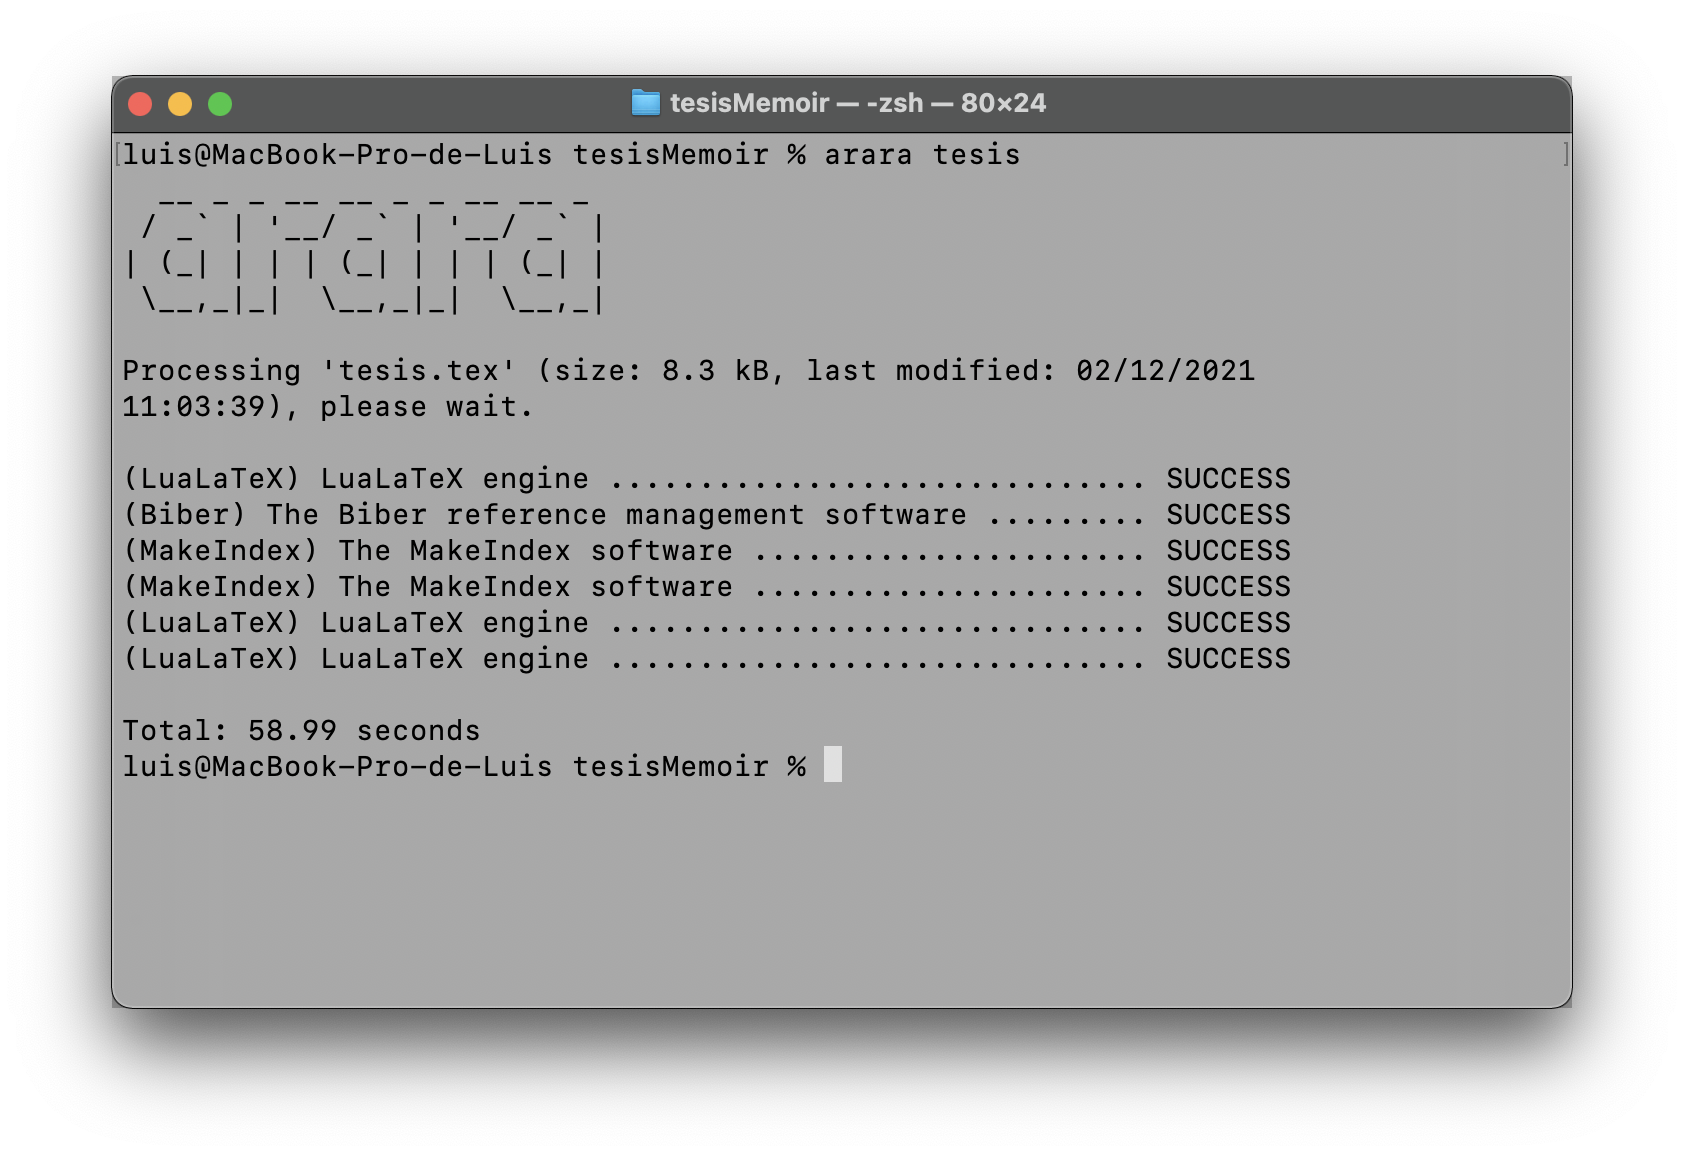
\includegraphics[scale=0.3]{primera}
  \caption{Primera compilación}
\end{figure}

\begin{figure}
\centering
  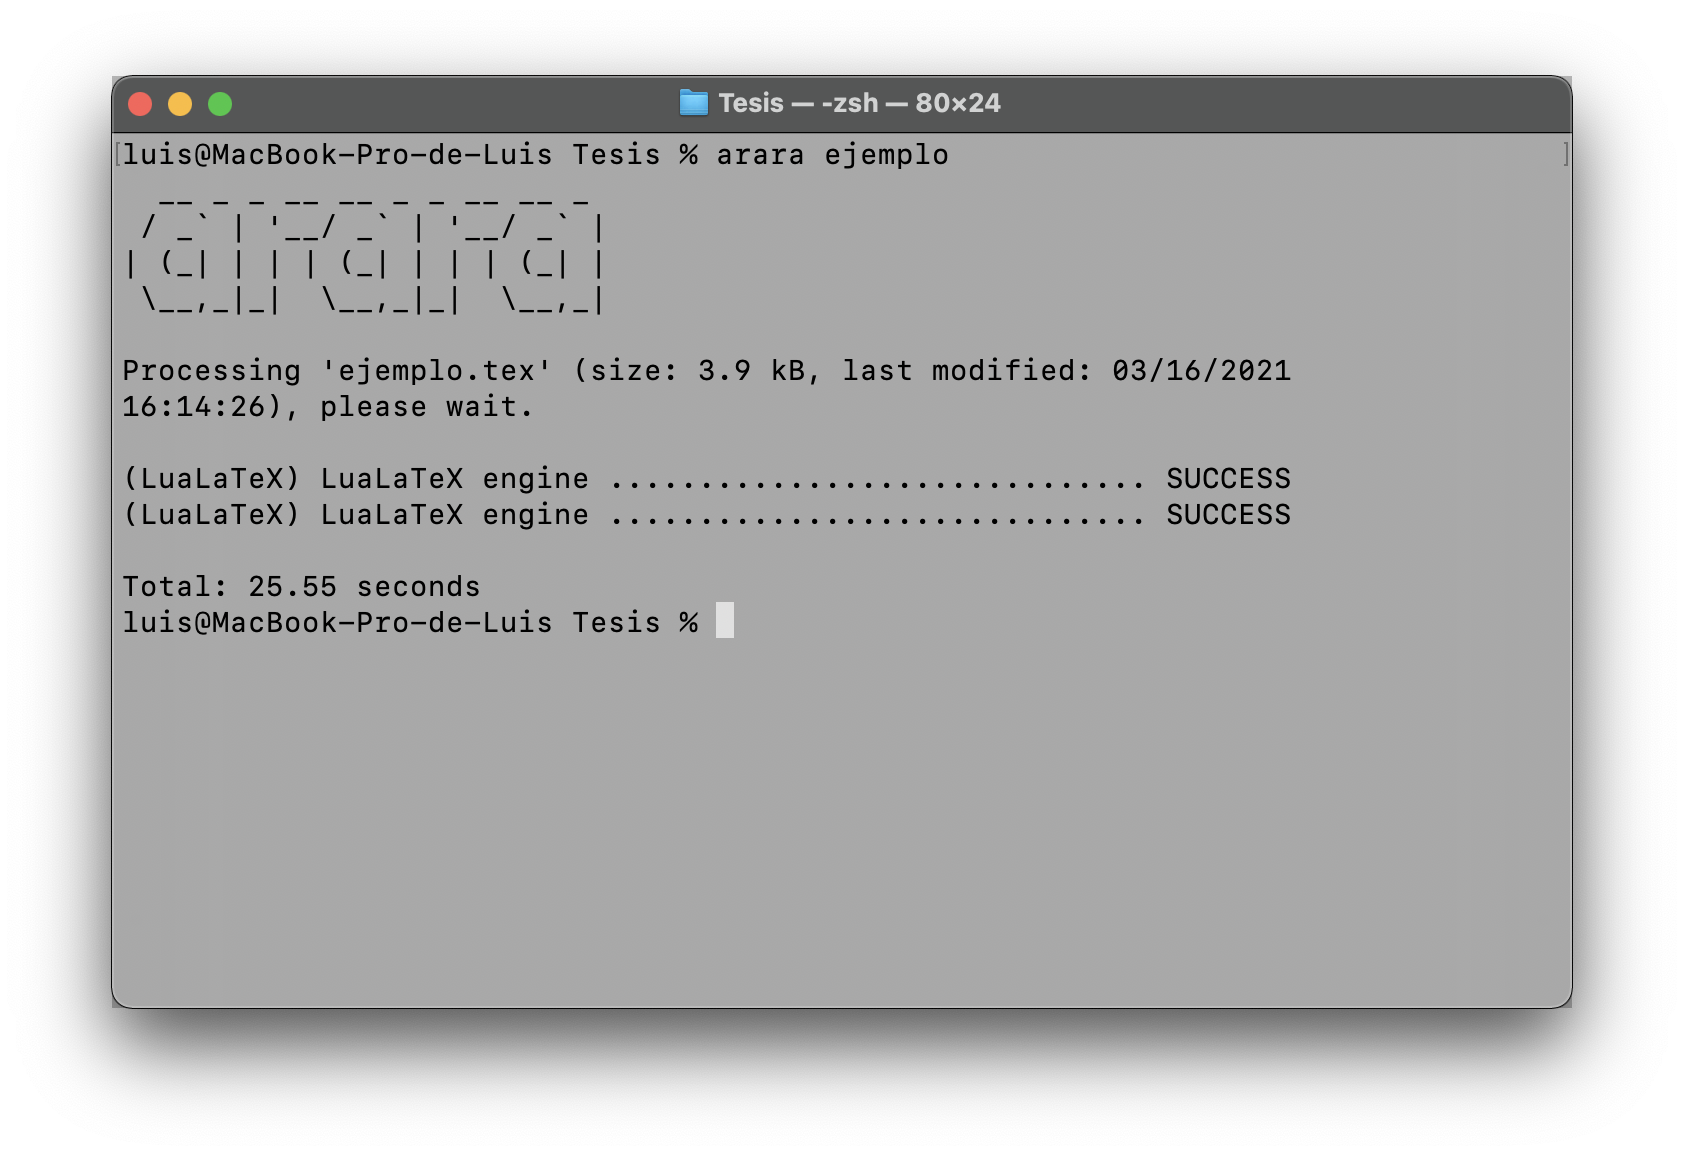
\includegraphics[scale=0.3]{segunda}
  \caption{Segunda compilación}
\end{figure}


%BIBLIOGRAFÍA
\backmatter%
\nocite{*}
\printbibliography%

%GLOSARIOS
\clearpage
\renewcommand{\preindexhook}{Se puede escribir algo antes de las entradas del índice}
\printindex

\clearpage
\renewcommand{\indexname}{Índice de nombres}
\renewcommand{\preindexhook}{}%Para que no ponga lo mismo que en el anterior
\printindex[names]

%\clearpage
%\renewcommand{\glossaryname}{Acrónimos}
%\printglossary[acro]
%
%\clearpage
%\renewcommand{\glossaryname}{Lista de símbolos}
%\printglossary[simb]


\end{document}
